\documentclass[a4paper]{article}
\usepackage[utf8]{inputenc}
\usepackage[russian,english]{babel}
\usepackage[T2A]{fontenc}
\usepackage[left=10mm, top=20mm, right=18mm, bottom=15mm, footskip=10mm]{geometry}
\usepackage{indentfirst}
\usepackage{amsmath,amssymb}
\usepackage[italicdiff]{physics}
\usepackage{graphicx}
\graphicspath{{images/}}
\DeclareGraphicsExtensions{.pdf,.png,.jpg}
\usepackage{wrapfig}

\usepackage{caption}
\captionsetup[figure]{name=Рисунок}
\captionsetup[table]{name=Таблица}

\begin{document}

\begin{wrapfigure}{R}{.3\textwidth}
    \centering
    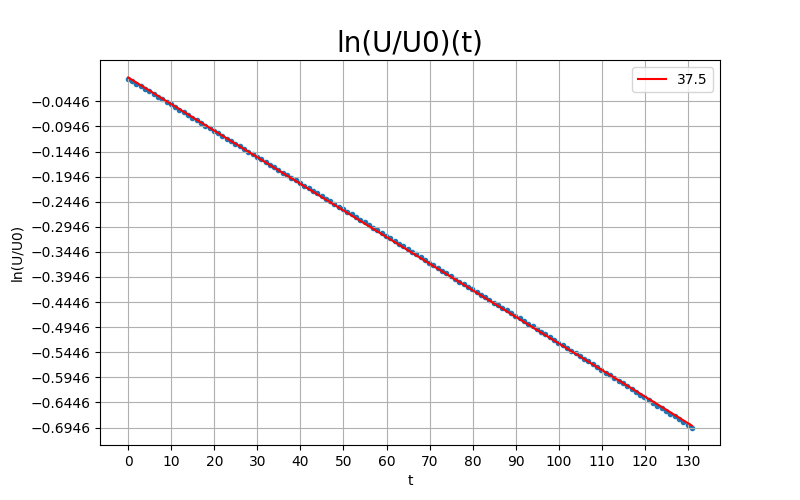
\includegraphics[width=0.8\textwidth]{37_5.png}
    \caption{Устройство}
\end{wrapfigure}
 

\begin{wrapfigure}{R}{.3\textwidth}
    \centering
    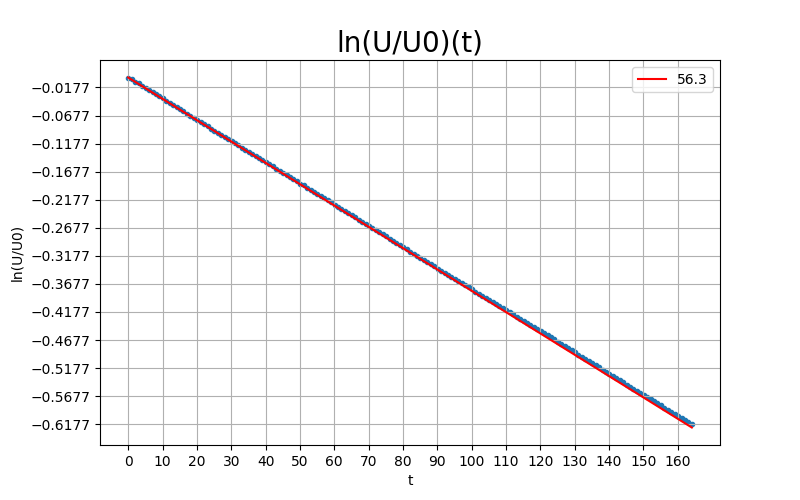
\includegraphics[width=0.8\textwidth]{56_3.png}
    \caption{Устройство}
\end{wrapfigure}

\begin{wrapfigure}{R}{.3\textwidth}
    \centering
    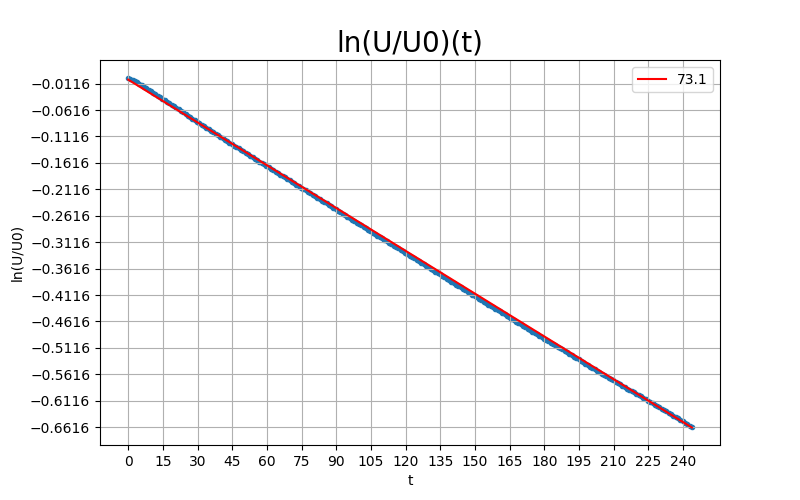
\includegraphics[width=0.8\textwidth]{73_1.png}
    \caption{Устройство}
\end{wrapfigure}

\begin{wrapfigure}{R}{.3\textwidth}
    \centering
    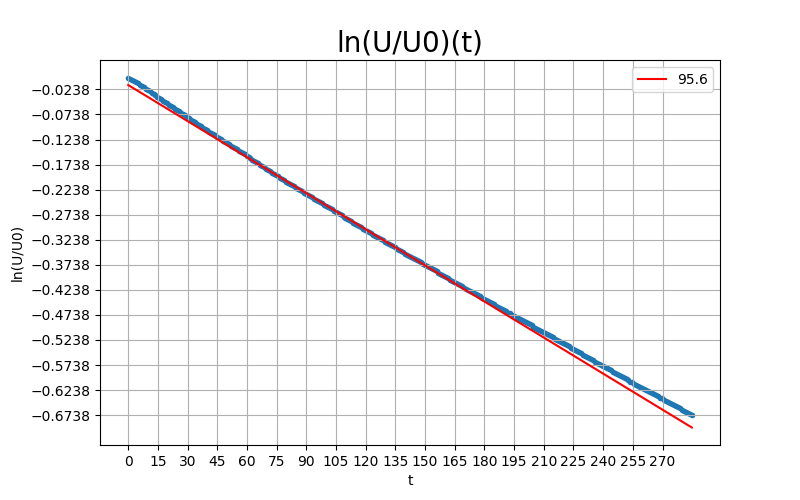
\includegraphics[width=0.8\textwidth]{95_6.png}
    \caption{Устройство}
\end{wrapfigure}

\begin{wrapfigure}{R}{.3\textwidth}
    \centering
    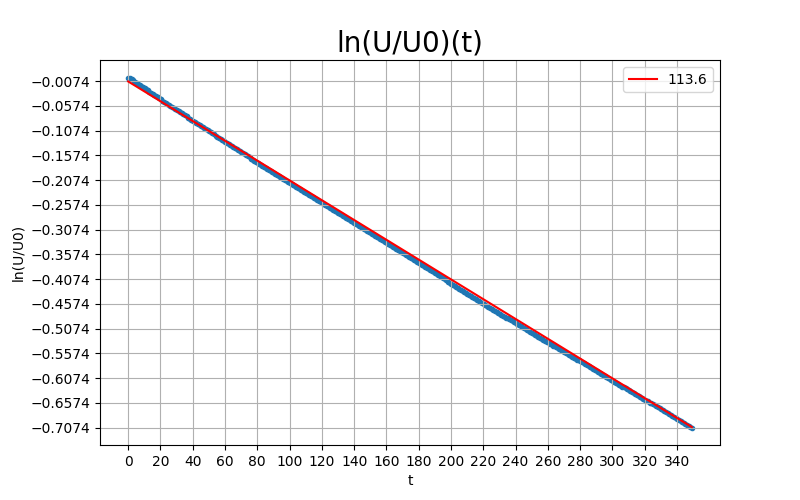
\includegraphics[width=0.8\textwidth]{113_6.png}
    \caption{Устройство}
\end{wrapfigure}

\begin{wrapfigure}{R}{.3\textwidth}
    \centering
    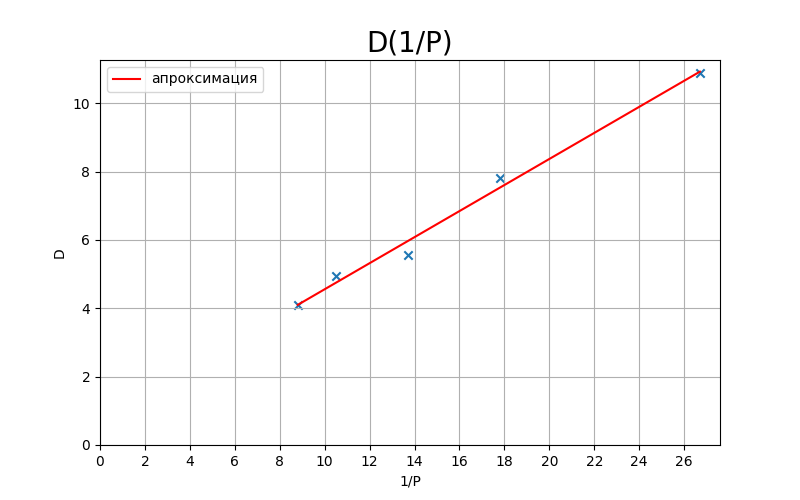
\includegraphics[width=0.8\textwidth]{DP.png}
    \caption{Устройство}
\end{wrapfigure}

\end{document}